%%
%% Automatically generated file from DocOnce source
%% (https://github.com/hplgit/doconce/)
%%
%%
% #ifdef PTEX2TEX_EXPLANATION
%%
%% The file follows the ptex2tex extended LaTeX format, see
%% ptex2tex: http://code.google.com/p/ptex2tex/
%%
%% Run
%%      ptex2tex myfile
%% or
%%      doconce ptex2tex myfile
%%
%% to turn myfile.p.tex into an ordinary LaTeX file myfile.tex.
%% (The ptex2tex program: http://code.google.com/p/ptex2tex)
%% Many preprocess options can be added to ptex2tex or doconce ptex2tex
%%
%%      ptex2tex -DMINTED myfile
%%      doconce ptex2tex myfile envir=minted
%%
%% ptex2tex will typeset code environments according to a global or local
%% .ptex2tex.cfg configure file. doconce ptex2tex will typeset code
%% according to options on the command line (just type doconce ptex2tex to
%% see examples). If doconce ptex2tex has envir=minted, it enables the
%% minted style without needing -DMINTED.
% #endif

% #define PREAMBLE

% #ifdef PREAMBLE
%-------------------- begin preamble ----------------------

\documentclass[%
oneside,                 % oneside: electronic viewing, twoside: printing
final,                   % draft: marks overfull hboxes, figures with paths
10pt]{article}

\listfiles               % print all files needed to compile this document

\usepackage{relsize,makeidx,color,setspace,amsmath,amsfonts,amssymb}
\usepackage[table]{xcolor}
\usepackage{bm,microtype}

\usepackage[pdftex]{graphicx}

\usepackage[T1]{fontenc}
%\usepackage[latin1]{inputenc}
\usepackage{ucs}
\usepackage[utf8x]{inputenc}

\usepackage{lmodern}         % Latin Modern fonts derived from Computer Modern

% Hyperlinks in PDF:
\definecolor{linkcolor}{rgb}{0,0,0.4}
\usepackage{hyperref}
\hypersetup{
    breaklinks=true,
    colorlinks=true,
    linkcolor=linkcolor,
    urlcolor=linkcolor,
    citecolor=black,
    filecolor=black,
    %filecolor=blue,
    pdfmenubar=true,
    pdftoolbar=true,
    bookmarksdepth=3   % Uncomment (and tweak) for PDF bookmarks with more levels than the TOC
    }
%\hyperbaseurl{}   % hyperlinks are relative to this root

\setcounter{tocdepth}{2}  % number chapter, section, subsection

% Tricks for having figures close to where they are defined:
% 1. define less restrictive rules for where to put figures
\setcounter{topnumber}{2}
\setcounter{bottomnumber}{2}
\setcounter{totalnumber}{4}
\renewcommand{\topfraction}{0.95}
\renewcommand{\bottomfraction}{0.95}
\renewcommand{\textfraction}{0}
\renewcommand{\floatpagefraction}{0.75}
% floatpagefraction must always be less than topfraction!
% 2. ensure all figures are flushed before next section
\usepackage[section]{placeins}
% 3. enable begin{figure}[H] (often leads to ugly pagebreaks)
%\usepackage{float}\restylefloat{figure}

% newcommands for typesetting inline (doconce) comments
\newcommand{\shortinlinecomment}[3]{{\color{red}{\bf #1}: #2}}
\newcommand{\longinlinecomment}[3]{{\color{red}{\bf #1}: #2}}

% prevent orhpans and widows
\clubpenalty = 10000
\widowpenalty = 10000

% --- end of standard preamble for documents ---


% insert custom LaTeX commands...

\raggedbottom
\makeindex

%-------------------- end preamble ----------------------

\begin{document}

% endif for #ifdef PREAMBLE
% #endif


% ------------------- main content ----------------------



% ----------------- title -------------------------

\thispagestyle{empty}

\begin{center}
{\LARGE\bf
\begin{spacing}{1.25}
FFM232, Klassisk fysik och vektorfält - Föreläsningsanteckningar
\end{spacing}
}
\end{center}

% ----------------- author(s) -------------------------

\begin{center}
{\bf \href{{http://fy.chalmers.se/subatom/tsp/}}{Christian Forssén}, Institutionen för fysik, Chalmers, Göteborg, Sverige${}^{}$} \\ [0mm]
\end{center}

\begin{center}
% List of all institutions:
\end{center}
    
% ----------------- end author(s) -------------------------

% --- begin date ---
\begin{center}
Sep 28, 2016
\end{center}
% --- end date ---

\vspace{1cm}


\section{Repetition: Singulära fält}

\paragraph{Punktkälla i origo.}
Fältet i punkten $\vec{r}$
\begin{equation}
  \vec{F}(\vec{r}) = \frac{q}{4 \pi r^2} \hat{e}_r,
\end{equation}
vilket fås av potentialen
\begin{equation}
  \phi(\vec{r}) = \frac{q}{4 \pi r},
\end{equation}
eftersom $\vec{F} = - \nabla \phi$.

Källtäthet $\rho (\vec{r}) = \nabla \cdot \vec{F} = - \Delta \phi$.

För detta fält insåg vi att det blir problem med Gauss sats
\begin{equation}
  \int_V \nabla \cdot \vec{F} \mbox{d}V = \oint_{\partial V} \vec{F} \cdot \mbox{d} \vec{S},
\end{equation}
eftersom $\nabla \cdot \vec{F} = 0$ skulle ge $\mathrm{VL} = 0$, men $\mathrm{HL} = q$ om den inneslutna volymen $V$ innehåller origo. Problemet är att 
\begin{equation}
\nabla \cdot \vec{F} = 
\left\{
\begin{array}{ll}
0 & r \neq 0 \\ 
\infty & r=0 
\end{array}
\right.
\end{equation}
En bättre beskrivning av en sådan källtäthet kommer härnäst...

\subsection{7. Deltafunktioner}

Kan vi approximera $\nabla \cdot \vec{F} = \rho (\vec{r})$ på något sätt? T.ex.
\begin{equation}
\rho = 
\left\{
\begin{array}{ll}
c & r < \varepsilon \\ 
0 & r > \varepsilon
\end{array}
\right.
\end{equation}
Dvs, en "utsmetad" punktladdning där vi väljer $c$ så att den totala laddningen är $q$, dvs
\begin{equation}
\rho = 
\left\{
\begin{array}{ll}
\frac{q}{\frac{4\pi}{3} \varepsilon^3} & r < \varepsilon \\ 
0 & r > \varepsilon
\end{array}
\right.
\end{equation}
\begin{itemize}
\item Vad blir gränsen då $\varepsilon \to 0^+$? 

\item Det kan vi tyvärr inte definiera.

\item $\rho(\vec{r}) = \lim_{\varepsilon \to 0^+} \rho_\varepsilon(\vec{r})$ är inte en funktion; sekvensen av funktioner som erhålls genom att variera $\varepsilon$ kallas för en distribution.
\end{itemize}

\noindent
\subsection{Deltafunktioner i en dimension}

\paragraph{Punktkälla i $D=1$.}
I en dimension kan vi definiera en punktkälla från potentialen
\begin{equation}
\phi(x) = -\frac{q}{2} \left| x \right|
\end{equation}



% inline figure
\centerline{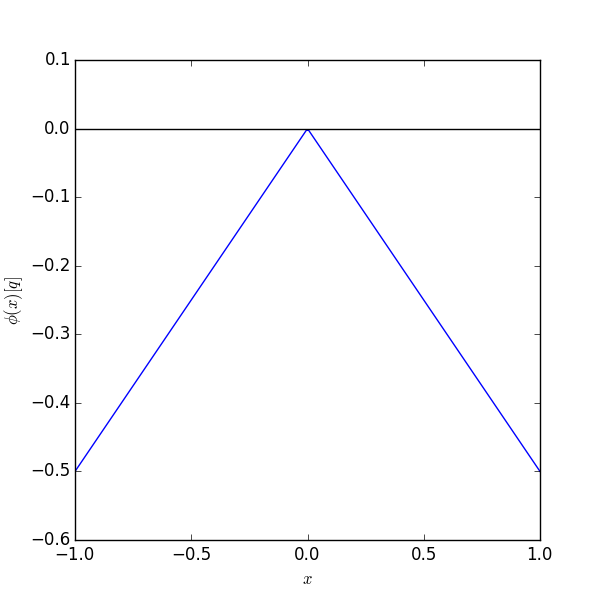
\includegraphics[width=0.8\linewidth]{fig/pointcharge_pot_1dim.png}}



vilket ger fältet
\begin{equation}
\vec{F}(x) = -\hat{x} \frac{\mbox{d}\phi}{\mbox{d}x} = 
\left\{
\begin{array}{ll}
\frac{q}{2} \hat{x} & x > 0 \\ 
-\frac{q}{2} \hat{x} & x < 0 \\ 
\end{array}
\right.
\end{equation}



% inline figure
\centerline{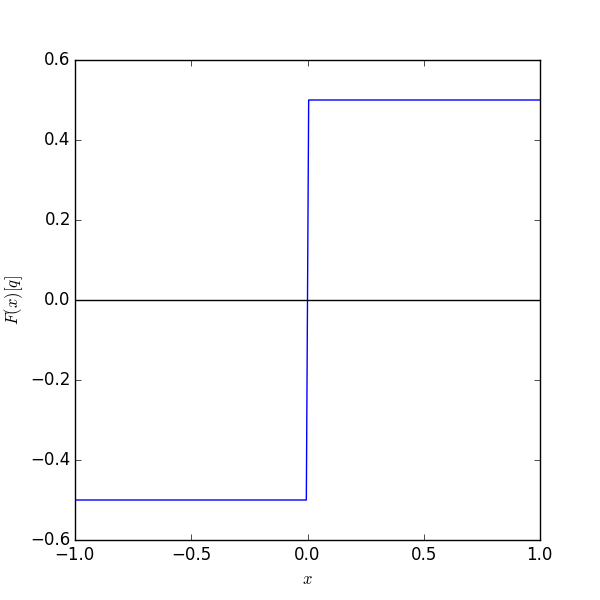
\includegraphics[width=0.8\linewidth]{fig/pointcharge_field_1dim.png}}



Vi kallar den enda komponenten av detta vektorfält för $F(x)$. Motsvarigheten till Gauss sats för detta endimensionella fält är 
\begin{equation}
\int_a^b \frac{\mbox{d}F}{\mbox{d}x} \mbox{d}x  = F(b) - F(a) = 
\left\{
\begin{array}{ll}
q, & \mathrm{om~} a < 0 < b \\ 
0, & \mathrm{annars} \\ 
\end{array}
\right.
\end{equation}
medan en naiv insättning av $\mbox{d}F / \mbox{d}x = 0$ i VL hade gett noll.

Problemet är ju att $\frac{\mbox{d}F}{\mbox{d}x} = 0$ för $x \neq 0$, men $\frac{\mbox{d}F}{\mbox{d}x} =  \infty$ för $x = 0$. Vi kan uttrycka detta som en "funktion", $\frac{\mbox{d}F}{\mbox{d}x} = q \delta(x)$, som är noll då $x \neq 0$ men som också uppfyller
\begin{equation}
\int_{a<0}^{b>0} \delta(x) \mbox{d}x = 1.
\end{equation}

\paragraph{Distributioner.}
Vi konstruerar denna "funktion" som en gräns $\varepsilon \to 0^+$ för
\begin{equation}
h_\varepsilon(x)
= 
\left\{
\begin{array}{ll}
0 & |x| > \frac{\varepsilon}{2} \\ 
\frac{1}{\varepsilon} & |x| < \frac{\varepsilon}{2} \\ 
\end{array}
\right.
\end{equation}



% inline figure
\centerline{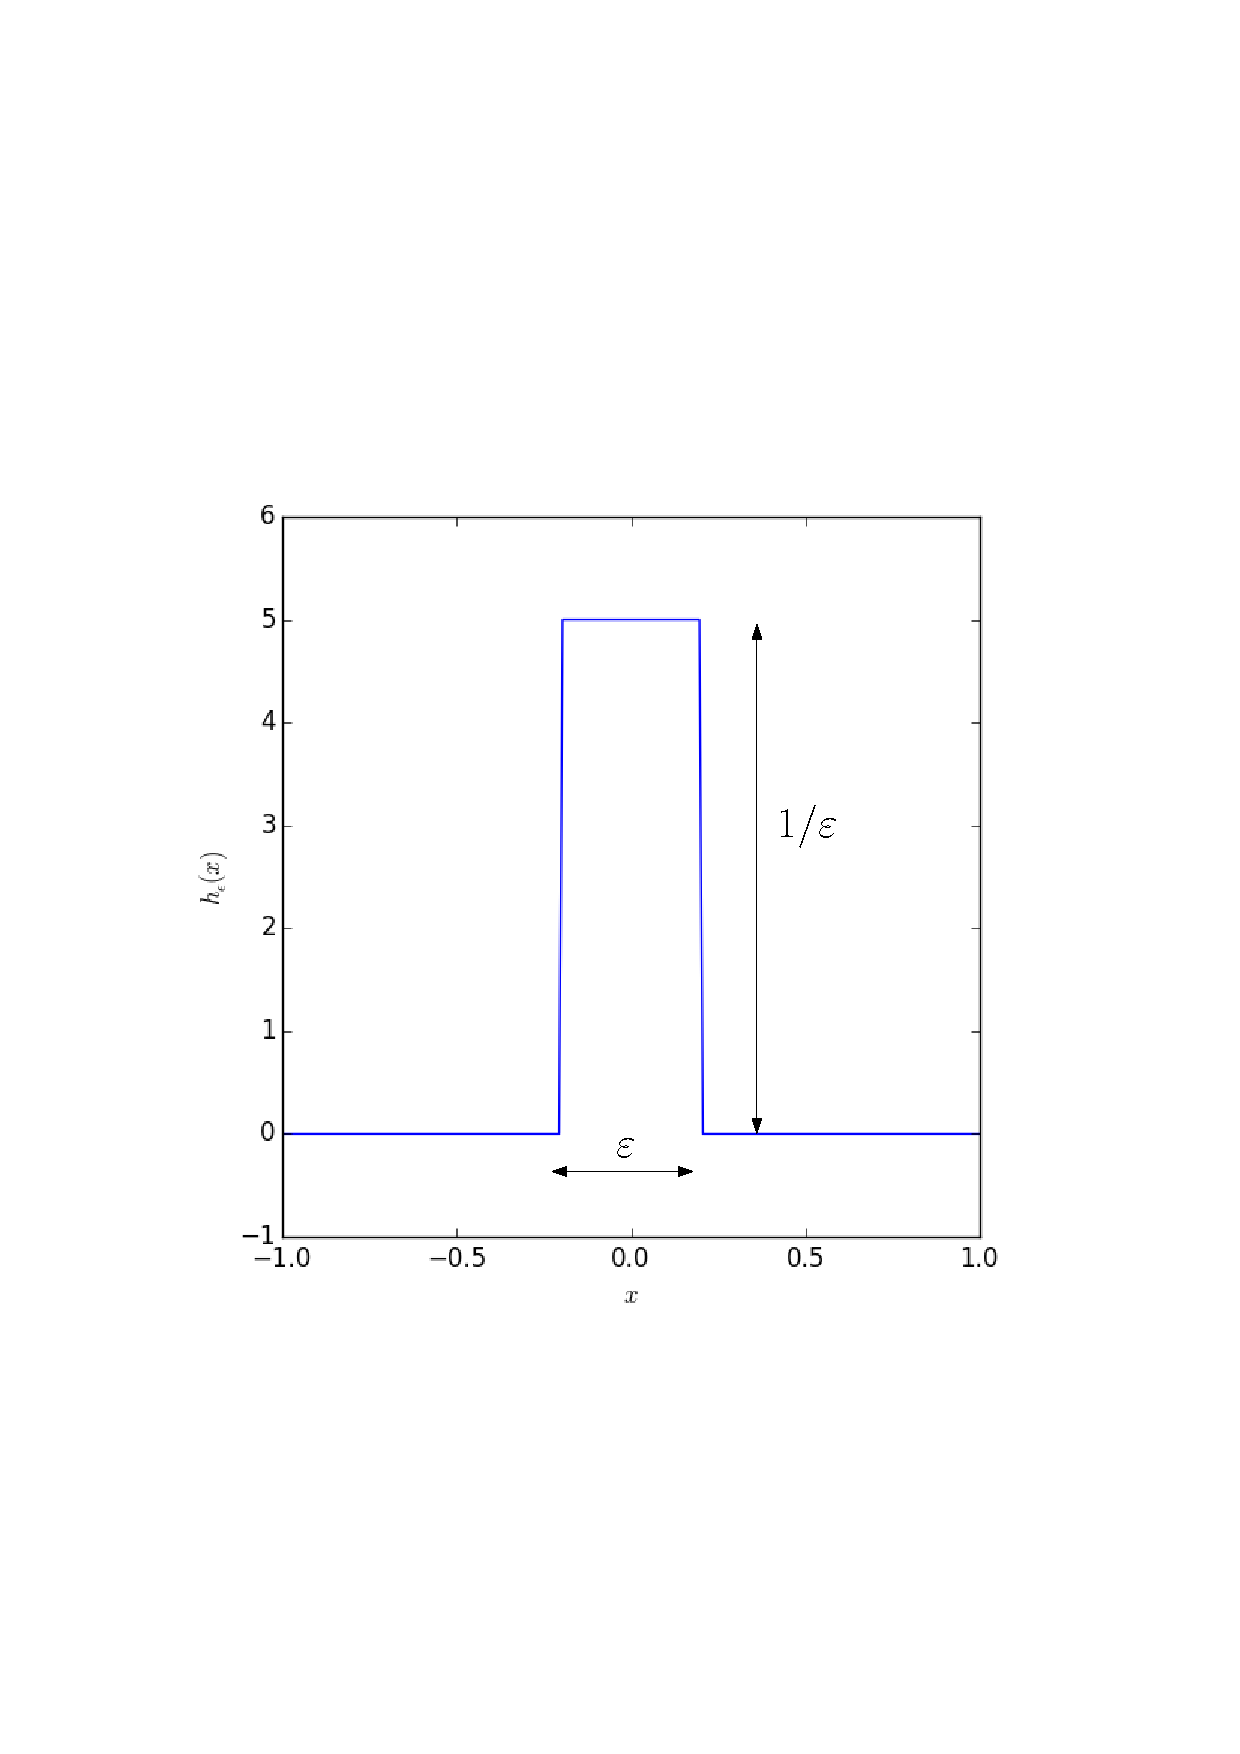
\includegraphics[width=0.8\linewidth]{fig/delta_step.pdf}}



\paragraph{Kontrollera.}
$$
\lim_{\varepsilon \to 0} h_\varepsilon(x) = 0,
$$
för $x \neq 0$. Dessutom har vi
$$
\lim_{\varepsilon \to 0} \int_{a<0}^{b>0} h_\varepsilon(x) \mbox{d}x 
= \lim_{\varepsilon \to 0} \int_{-\varepsilon/2}^{\varepsilon/2} \frac{1}{\varepsilon} \mbox{d}x
= \lim_{\varepsilon \to 0} 1 = 1.
$$
---------------------------------------

Men det finns också andra möjligheter
\begin{align}
h_\varepsilon(x) &= \frac{\exp(-x^2 / \varepsilon^2)}{\sqrt{\pi} \varepsilon}, \\ 
h_\varepsilon(x) &= \frac{\varepsilon}{\pi (x^2 + \varepsilon^2)}, \\ 
h_\varepsilon(x) &= \frac{\sin(x/\varepsilon)}{\pi x} \label{eq:sinxdelta}.
\end{align}




% inline figure
\centerline{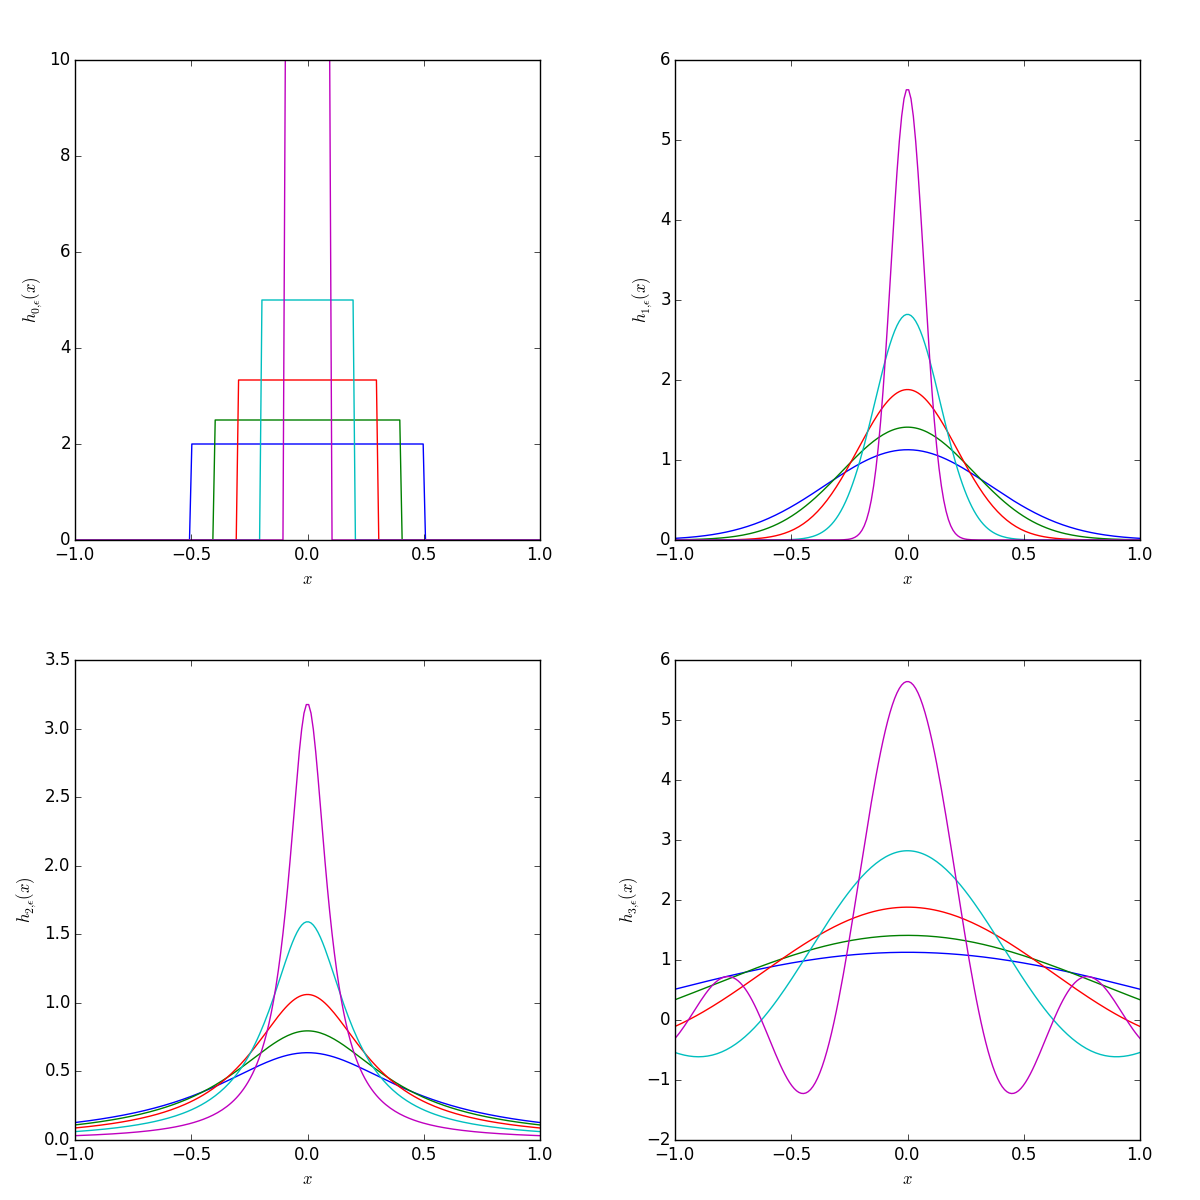
\includegraphics[width=0.95\linewidth]{fig/deltas.png}}



Samtliga dessa utgör en \emph{sekvens av funktioner} (en \emph{distribution}) från vilka vi kan definiera \emph{Diracs deltafunktion}
\begin{equation}
\delta(x) = \lim_{\varepsilon \to 0^+} h_\varepsilon(x)
\end{equation}
med de definierande egenskaperna
\begin{align}
\delta(x) &= 0, \quad x \neq 0 \\ 
f(0) &= \int_a^b f(x) \delta(x) \mbox{d}x,
\end{align}
där $f(x)$ är en välbeteende funktion och $\left[ a,b \right]$ inkluderar 0. Ett specialfall av ovanstående är
\begin{equation}
\int_{-\infty}^{+\infty} \delta(x) \mbox{d}x = 1
\end{equation}

------------------------------

\paragraph{Exempel.}
-----------------------

Kontrollera att vi erhåller Diracs deltafunktion från sekvensen $h_\varepsilon(x) = \frac{\exp(-x^2 / \varepsilon^2)}{\sqrt{\pi} \varepsilon}$.

\emph{Lösning}:
För $x \neq 0$ gäller
\begin{align}
h_\varepsilon(x) 
&= \frac{1}{\sqrt{\pi} \varepsilon \exp(x^2 / \varepsilon^2)}
= \frac{1}{\sqrt{\pi} \varepsilon \left[ 1 + \frac{x^2}{\varepsilon^2} + \frac{1}{2}\left(\frac{x^2}{\varepsilon^2}\right)^2 + \ldots \right] } \nonumber \\ 
&= \frac{\varepsilon}{\sqrt{\pi}} \frac{1}{\left( x^2 + \varepsilon^2 + \frac{x^4}{2\varepsilon^2} + \ldots \right)} \to 0 \quad \mathrm{då~} \varepsilon \to 0^+
\label{eq:heps0}
\end{align}
Vidare har vi integralen $\int_{-\infty}^\infty e^{-x^2 / \varepsilon^2} \mbox{d}x = \sqrt{\pi \varepsilon^2}$ (se tabell över definita integraler, eventuellt Beta 7.5-41). Detta ger
\begin{equation}
\lim_{\varepsilon \to 0^+}
\int_{-\infty}^{+\infty} \frac{\exp(-x^2 / \varepsilon^2)}{\sqrt{\pi} \varepsilon} \mbox{d}x = \lim_{\varepsilon \to 0} \frac{\sqrt{\pi \varepsilon^2}}{\sqrt{\pi} \varepsilon} = 1, \quad \mathrm{för~} \varepsilon>0.
\label{eq:heps1}
\end{equation}
För att vara helt korrekta skall vi egentligen visa den mer allmänna egenskapen $\int_a^b f(x) \delta(x) \mbox{d}x = f(0)$ för en väl beteende funktion $f(x)$. Eftersom ekv. (\ref{eq:heps0}) gäller, och $f(x)$ inte utgör något problem, kan vi utöka integrationsintervallet och istället studera
\begin{equation}
\int_{-\infty}^{+\infty} f(x) \delta(x) \mbox{d}x = f(0).
\end{equation}
Vi Taylorutvecklar, $f(x) = f(0) + f'(0)x + f''(0)x^2/2+\ldots$, och konstaterar att 

\begin{equation}
\lim_{\varepsilon \to 0} \int_{-\infty}^{+\infty} f(0) h_\varepsilon(x) \mbox{d}x = f(0) \lim_{\varepsilon \to 0} \int_{-\infty}^{+\infty} h_\varepsilon(x) \mbox{d}x = f(0),
\end{equation}
enligt vad vi visat ovan (\ref{eq:heps1}). Det återstår att visa att 
\begin{equation}
\lim_{\varepsilon \to 0} \int_{-\infty}^{+\infty} x^n h_\varepsilon(x) \mbox{d}x = 0,
\label{eq:xnheps0}
\end{equation}
för alla heltal $n>0$. I vårt fall har vi en jämn funktion $h_\varepsilon(x)$ vilket gör att ekv. (\ref{eq:xnheps0}) är trivialt uppfyllt för udda $n$ då integranden blir udda. För jämna $n=2k$ finner vi (se t.ex. Beta 7.5-42) 
\begin{equation}
\lim_{\varepsilon \to 0^+}
\int_{-\infty}^{+\infty} x^{2k} \frac{\exp(-x^2 / \varepsilon^2)}{\sqrt{\pi} \varepsilon} \mbox{d}x = \lim_{\varepsilon \to 0} \frac{2}{\sqrt{\pi} \varepsilon} \frac{(2k-1)!!}{2^{k+1}} \sqrt{\pi} \varepsilon \varepsilon^{2k} = 0, \quad \mathrm{för~} \varepsilon>0.
\end{equation}
Alltså har vi visat att
\begin{equation}
\lim_{\varepsilon \to 0^+}
\int_{a<0}^{b>0} f(x) \frac{\exp(-x^2 / \varepsilon^2)}{\sqrt{\pi} \varepsilon} \mbox{d}x = f(0), \quad \mathrm{för~} \varepsilon>0.
\end{equation}

-----------------------------------------------

\subsection{Egenskaper hos Diracs deltafunktion}

\begin{itemize}
\item Jämn: $$\delta(-x) = \delta(x)$$

\item Skalning: 
\end{itemize}

\noindent
$$
\delta(ax) = \frac{1}{|a|} \delta(x).
$$ 

\longinlinecomment{Comment 1}{ Visas enklast genom att göra substitutionen $y=x a$ i uttrycket $\int_{-\infty}^{+\infty} f(x) \delta(ax) \mbox{d}x$. Var noga med tecknet på integrationsgränserna. }{ Visas enklast genom att }
\begin{itemize}
\item Translation: 
\end{itemize}

\noindent
$$
\int_{-\infty}^{+\infty} f(x) \delta(x-x_0) \mbox{d}x = f(x_0).
$$
\shortinlinecomment{Comment 2}{ visas genom substitutionen $y=x-x_0$. }{ visas genom substitutionen $y=x-x_0$. }
\begin{itemize}
\item Derivata 
\end{itemize}

\noindent
$$
\int_{-\infty}^{+\infty} f(x) \delta'(x-x_0) \mbox{d}x = -\int_{-\infty}^{+\infty} f'(x) \delta(x-x_0) \mbox{d}x = -f'(x_0),
$$
vilket kan betraktas som definitionen av derivatan $\delta'(x)$.

\shortinlinecomment{Comment 3}{ Visas genom partiell integration med någon av funktionssekvenserna som definierar deltafunktionen. }{ Visas genom partiell integration }
\begin{itemize}
\item Kan generaliseras till andra dimensioner. Vi skriver generellt $\delta^{(D)}(\vec{r})$, där vi skall tolka superskriptet som antalet dimensioner. T.ex. har vi för $D=3$ 
\end{itemize}

\noindent
$$
\delta^{(3)}(\vec{r}) = \delta(x) \delta(y) \delta(z).
$$
I sfäriska koordinater blir detta
$$
\iiint f(\vec{r}) \delta^{(3)}(\vec{r} - \vec{r}_0) r^2 \sin\theta \mbox{d}r \mbox{d}\theta \mbox{d}\phi = f(\vec{r}_0).
$$
Med vissa förbehåll kan deltafunktionen i kroklinjiga koordinater skrivas
$$
\delta^{(3)}(\vec{r} - \vec{r}_0) = \frac{1}{h_1(\vec{r}_0) h_2(\vec{r}_0) h_3(\vec{r}_0)} \delta(u_1-u_{1,0}) \delta(u_2-u_{2,0}) \delta(u_3-u_{3,0}).
$$

\subsection{Deltafunktioner i högre dimensioner}

Vi startar med punktkällan i origo: $\vec{F} = \frac{q}{4 \pi r^2} \hat{e}_r$, och den problematiska volymsintegralen
$$
\int_V \nabla \cdot \vec{F} \mbox{d}V,
$$
som borde bli lika med $q$ om $V$ omfattar origo. Detta kan vi åstadkomma genom att införa $\nabla \cdot \vec{F} = q \delta^3(x) = q \delta(x)\delta(y)\delta(z)$ eftersom
$$
\iiint \mbox{d}x \mbox{d}y \mbox{d}z \delta(x)\delta(y)\delta(z) = 1.
$$
Ännu bättre blir det om vi jobbar konsekvent med sfäriska koordinater. Inför ett \emph{regulariserat} fält
\begin{equation}
\vec{F}_\varepsilon(\vec{r}) = \frac{q}{4 \pi (r^2 + \varepsilon^2)} \hat{e}_r
\end{equation}
som uppenbarligen går mot $\vec{F}$ då $\varepsilon \to 0^+$.

Divergensen blir ($\nabla \cdot \vec{F} = \frac{1}{r^2} \frac{\partial}{\partial r} (r^2 F_r) + \ldots$)
\begin{align}
\nabla \cdot \vec{F}_\varepsilon(\vec{r}) &= \frac{q}{4 \pi r^2} \underbrace{\frac{\partial}{\partial r} \left( \frac{r^2}{r^2 + \varepsilon^2} \right)}_{=\frac{2r}{r^2 + \varepsilon^2} - \frac{2 r r^2}{(r^2 + \varepsilon^2)^2} = \frac{2 r \varepsilon^2}{(r^2 + \varepsilon^2)^2}} \\ 
&= \frac{q \varepsilon^2}{2 \pi} \frac{1}{r(r^2 + \varepsilon^2)^2} \to 0 \quad \mathrm{då} \; \varepsilon \to 0.
\end{align}
Utan styrkan $q$ kallar vi denna sekvens av funktioner för $h_\varepsilon(\vec{r})$ och påstår att $\lim_{\varepsilon \to 0} h_\varepsilon(\vec{r}) = \delta^3(\vec{r})$. Utför integralen
\begin{align}
\int_V \nabla \cdot \vec{F}_\varepsilon \mbox{d} V &= \int_V q h_\varepsilon(\vec{r}) \mbox{d} V = \frac{ q \varepsilon^2}{2 \pi} 4\pi \int_0^\infty r^2 \mbox{d} r \frac{1}{r(r^2 + \varepsilon^2)^2} \\ 
&= 2 q \varepsilon^2 \left[ -\frac{1}{2} \frac{1}{r^2 + \varepsilon^2} \right]_0^\infty = 2 q \varepsilon^2 \frac{1}{2 \varepsilon^2} = q
\end{align}
Alltså har vi visat att
\begin{itemize}
\item $\lim_{\varepsilon \to 0} h_\varepsilon(\vec{r}) = 0$ för $r \neq 0$.

\item $\int_{\mathbf{R}^3} h_\varepsilon(\vec{r}) \mbox{d}V = 1$
\end{itemize}

\noindent
Alltså skriver vi källtätheten 
$$
\rho(\vec{r}) = \nabla \cdot \vec{F} = -\Delta \phi = q \delta^3(\vec{r}).
$$

\paragraph{Linjekälla.}
Linjekällan $\vec{F} = \frac{k}{2 \pi \rho} \hat{e}_\rho$ (motsvarar en punktkälla i $D=2$).
Källtätheten kan skrivas
$$
\nabla \cdot \vec{F} = k \delta^2(\vec{\rho}) \left( = k \delta(x) \delta(y) \right).
$$
Studera t.ex. normalytintegralen genom en cylinder med höjden $L$ runt linjekällan
$$
\int_S \vec{F} \cdot \mbox{d}\vec{S} = \int_{S+S_0+S_L} \vec{F} \cdot \mbox{d}\vec{S} = \int_V \nabla \cdot \vec{F} \mbox{d} V = \int_0^L \mbox{d} z \int \mbox{d}x \mbox{d}y k \delta(x)\delta(y) = \int_0^L \mbox{d} z k = k L.
$$
där vi först har slutit ytan genom att införa ytorna $S_0$ och $S_L$ som är cirkelskivor vid botten och toppen och som har normalytintegralen noll eftersom fältet är vinkelrät mot normalen.

\paragraph{Virveltråd.}
Vi kan resonera på liknande sätt för en virveltråd $\vec{F} = \frac{J}{2 \pi \rho} \hat{e}_\phi$. Stokes sats säger att
$$
\int_{\partial S} \vec{F} \cdot \mbox{d} \vec{r} = \int_S (\nabla \times \vec{F}) \cdot \mbox{d} \vec{S},
$$
där vi kan räkna ut $\mathrm{VL} = J$ (t.ex. för en cirkel runt virveltråden). För detta fält är det rotationen som är problematisk. Notera att detta är en vektor.
$$
\nabla \times \vec{F} = J \delta^2(\vec{\rho}) \hat{z} = \vec{J} \delta(x)\delta(y).
$$

\paragraph{Exempel: tillämpning av deltafunktionen; Fouriertransform och ortogonalitet.}
-----------------------

Givet en funktion $f(x)$ definieras dess Fouriertransform som
$$
\tilde f(k)=\frac{1}{\sqrt{2\pi}}\int_{-\infty}^\infty dx\,e^{-ikx}f(x)
$$
Den inversa transformen ger frekvenssönderläggningen av $f(x)$, i detta fall motsvaras ``frekvensen'' av vågtalet $k$:
$$
f(x)=\frac{1}{\sqrt{2\pi}}\int_{-\infty}^\infty dk\,e^{ikx}\tilde f(k)
$$
(normeringen har valts för att åstadkomma symmetri mellan de två uttrycken).

Genom att sätta in det första uttrycket i det andra får man, under förutättning att man kan byta integrationsordning,
$$
f(x)=\frac{1}{\pi}\int_{-\infty}^\infty dk\,e^{ikx}
\int_{-\infty}^\infty dx'\,e^{-ikx'}f(x')=
\frac{1}{2\pi}\int_{-\infty}^\infty dx'
\left(\,\int_{-\infty}^\infty dk\,e^{ik(x-x')}\right)f(x')
$$

Uttrycket inom parenteser i det sista ledet beror bara på $x-x'$, och om resultatet skall bli $f(x)$ måste det vara en deltafunktion lika med $2\pi\delta(x-x')$. Dvs
\begin{equation}
\delta(x-x') = \frac{1}{2\pi} \int_{-\infty}^\infty dk\,e^{ik(x-x')}.
\label{eq:expdelta}
\end{equation}
Genom att byta vågtalet $k$ och koordinaten $x$ får man också $2\pi \delta(k-k') = \int_{-\infty}^\infty dx\,e^{i(k-k')x}$. Detta sätt att skriva deltafunktionen kunde vi också ha anat från ekv. (\ref{eq:sinxdelta}) genom att byta 
$$
\lim_{\varepsilon \to 0} \frac{\sin(x/\varepsilon)}{\pi x} \Rightarrow \lim_{n \to \infty} \frac{\sin(n x)}{\pi x}.
$$
Här kan man nämligen göra omskrivningen
\begin{equation}
\int_{-n}^n e^{i x t} dt = \left[ \frac{e^{ixt}}{ix} \right]_{-n}^n 
= \left[ \frac{\cos(xt)+i\sin(xt)}{ix} \right]_{-n}^n 
= 2 \frac{\sin(nx)}{x},
\end{equation}
så att vi får
\begin{equation}
\delta(x) = \lim_{n \to \infty} \frac{1}{2\pi} \int_{-n}^n e^{i x t} dt,
\end{equation}
vilket är analogt med ekv. (\ref{eq:expdelta})

Funktionerna $e_k(x)=\frac{1}{\sqrt{2\pi}}e^{ikx}$ kan alltså ses som ortogonala och ``deltafunktionsnormerade'' med ortogonalitetsrelationen
$$
\int_{-\infty}^\infty dx\,e^{\mathstrut}_k(x)e^*_{k'}(x)=\delta(k-k')
$$

Man kan bekräfta resultatet genom att göra beräkningen explicit 
för de regulariserade funktionerna $e_{k,\varepsilon}(x)={1\over\sqrt{2\pi}}e^{ikx-\varepsilon^2x^2}$ och låta $\varepsilon\rightarrow0$ (se uppgift 7.15). 

----------------------------------------------

% ------------------- end of main content ---------------


% #ifdef PREAMBLE
\printindex

\end{document}
% #endif

